\chapter{Results and Discussion}
\label{chap:Results_and_Discussion}

This chapter presents and analyzes the results of the implementation of the developed MPC framework on two different benchmarks. The first benchmark is the simulator for a well known tank system present here at the Control labs. This system was developed as a small test platform of the software before using it on the quadrotor simulator. The second benchmark is the simulator for the quadrotor, which comes from the modeling effort made in chapter 3. For each case, the structure to present the results will be divided in three sections: Simulation settings and parameters, Results and Discussion.

\section{Tank system simulations}

\subsection{Simulation settings and parameters}

The tank system's equations were provided with their correspondent identified parameters. The system is made of two tanks that are connected by gravity: one tank provides the inflow for the other and from there to a water deposit. There is also a small pump, its operation voltage represents the input to the system. The states of the system are the two tank level, of which the desired output is the level of the second  tank.  The system is depicted below as in Figure 5.1: 

\begin{figure}[H]
\centering
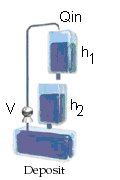
\includegraphics[scale=0.7]{Images/Chapter5/tank_system.png}
\caption{Representation of the tank system.}
\label{fig:tank_system}
\end{figure}

The constraints on the system arise from the size of the tanks, which limit the level of water that the system can handle. The constraints for the levels of the tanks, $H_1$ and $H_2$ respectively, and the input voltage are shown below:

\begin{table}[h]
\centering
 \begin{tabular}{ l }
   0 \leq H_1 \leq 25 [cm]   \\
   0 \leq H_2 \leq 28 [cm]  \\
   0 \leq V \leq 10 [V]
 \end{tabular} 
\end{table}

Regarding the tuning of MPC, the parameters available to adjust are the horizons and the weight matrices in the cost function. The selection of a proper prediction horizon for any MPC application is dependant on the dynamics of the system that is being controlled.  This choice is of great influence in the size of the optimization problem to solve, and therefore in the computational power required to provide deterministic operation. If the horizon is too short, the prediction will not give information about future control signals and might create unstability in the controller \cite{Gabrielsson2012}. On the other hand, if the horizon is too long, the optimization problem to solve could be too large to solve in each time sample, depending on the timing requirements for each case. The selected prediction horizon of 10 samples at a rate of 100 Hz was obtained starting from small values, where the optimization problems were mostly unfeasible, and increasing until feasibility was achieved, as well as a decent control signal. Further tuning is made with the weight matrices. The weight matrices are also selected in a trial and error fashion. \\

The specifications for the simulation of the MPC on the tank system is presented below.

\begin{table}[h]
\centering
\begin{tabular}{| l | l |}
    \hline
    Prediction horizon & 10 samples at a frequency of 100 Hz                                                                                                         \\ \hline
    Weight matrices & Specified in Appendix A                                                                                                                                      \\ \hline
    Input constraints & 0 \leq V \leq 10 [V]                                                                                                                                               \\ \hline
    State constraints & \begin{tabular}[c]{@{ }l@{}} 0 \leq H_1 \leq 25 [cm]  \\ 0 \leq H_2 \leq 28 [cm]  \end{tabular} \\ \hline
    Processor & Intel \textsuperscript{\textregistered} Core\texttrademark 2 Duo @ 3.0 GHz                                            \\ \hline
\end{tabular}
\end{table}

\subsection{Results}

The results of the simulation of the tank system under the MPC controller are shown below. 

\begin{figure}[H]
\centering
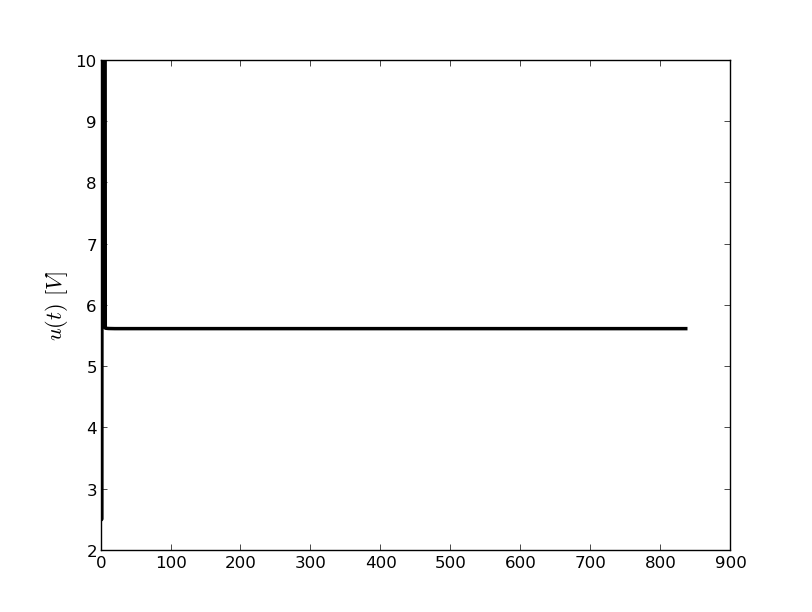
\includegraphics[scale=0.7]{Images/Chapter5/tank_system/control_signal.png}
\caption{Voltage inputs calculated for the tank system by the MPC controller.}
\label{fig:tanks_inputs}
\end{figure}

\begin{figure}[H]
\centeringState
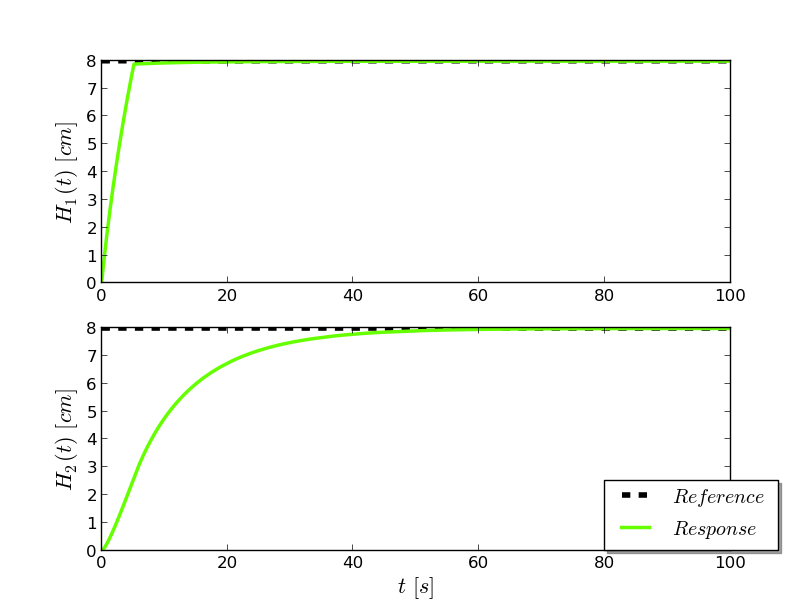
\includegraphics[scale=0.7]{Images/Chapter5/tank_system/levels_control.png}
\caption{Reference level and actual level of the simulated tanks.}
\label{fig:tanks_states}
\end{figure}

\subsection{Discussion}

Directly from Figures \ref{fig:tanks_inputs} and \ref{fig:tanks_states}, it is easy to see the controller acting on the input voltage and its influence on the tank states. Since this is a regulation problem for a relatively simple process, the MPC's features are not giving any advantage in comparison with standard PID controllers. However, due to the receding horizon the controller can introduce a feed forward action in a more natural way and can react better to disturbances than a classic controller. In Figure \ref{fig:tanks_inputs} the input constraint takes effect, limiting effectively the input voltage to the pump to 10 volts. It is important to notice that the output variable, $H_2$, takes some time to get to the required setpoint because the speed at which it can be filled is limited by Torricelli's principle for fluids flowing out under the sole influence of atmospherical pressure from a tank. However, level $H_1$ does rise quickly as the pump sends enough water to fill the tank to the point where the maximum flow of water out of it is achieved. 


\section{Quadrotor simulations}

\subsection{Simulation settings and parameters}

Since the quadrotor has only four actuators to move in six degrees of freedom, it is by definition, an underactuated system. Hence, there will be only four variables that will be controllable. The choice made was to control the $x, y, z$ positions and the orientation around the $z$ axis ($\psi$). It is important to mention that the MPC is not sending directly the input signals to the motors. The reason for this is that the model that is being used to perform the calculations is a linearized model, therefore the state and input variables represent deviations around an operation point. The MPC is instead controlling these linearized input variables and sending that to modify the initial operation point. The operation point being used is calculated by simple force balance in the hover condition, to obtain the required angular speed of the rotors to keep the quadrotor static in the air, which is approximately $360$ radians per second. That way, the control signal vector going to the quadrotor simulator is built as follows:

\begin{equation*}
\mathbf{u} = \underbrace{\mathbf{\bar{u}}}_\textrm{operation point} + \underbrace{\Delta \mathbf{u}}_\textrm{controlled by MPC}
\end{equation*}

In order to adjust to this, the constraints in the input were also modified, through a displacement of the operation range for this variation of the angular speed. The original operation range is taken from the experiments realized by Sun \cite{YueSun2012}, which is $130 \leq \omega_{i} \leq 500$, in radians per second. In order to be congruent with that range, the variation of the angular speed is limited between $-230 \leq \Delta \omega_{i} \leq 140$ around the operation point, again in radians per second.\\ 

In this particular case, the tuning of the MPC is also influenced by the model, since the one being used for prediction is a linearized version. A very long prediction in the future might mean moving too far away from the operation point, which will cause erratic predictions due to nonlinearities, additionally to the increase of the computation time. Also, these erratic prediction may lead the controller to unfeasibility and therefore unstability. In this system that is not stable in open loop, this could mean crashing the quadrotor. The selected prediction horizon of 30 samples at a rate of 120 Hz is long enough to give good predictions ahead for the system while keeping the problem at a reasonable size. This  result was obtained by trial and error.\\

With the weight matrices, the procedure is also made in a trial and error fashion. A good initial guess for the quadrotor model is taken from previous implementation parameters \cite{Bouffard2012}. The simulation is performed in a computer with an Intel \textsuperscript{\textregistered} Core\texttrademark 2 Duo running at 3.0 GHz. The complete specifications for the simulation are presented in the following table.

\begin{table}[h]
\begin{center}
    \begin{tabular}{| l | l |}
    \hline
    Prediction horizon & 30 samples at a frequency of 120 Hz \\ \hline
    Weight matrices & Specified in Appendix A \\ \hline
    Input constraints &  -230 \leq \Delta \omega_{i} \leq 140 [rad/s] \\ \hline 
    State constraints &  \begin{tabular} [c]{ @ {} l @{} } -5 \leq V_x \leq 5 [m] \\  -5 \leq V_y \leq 5 [m] \\ 0 \leq z \leq 5 [m] \end{tabular} \\ \hline
    Processor & Intel \textsuperscript{\textregistered} Core\texttrademark 2 Duo @ 3.0 GHz \\  \hline
    \end{tabular}
\end{center}
\end{table}

The trajectory reference used to test the MPC in the quadrotor simulator is based in simple decoupled movements in each one of the controlled directions, done one at a time. The movement consists in four stages: elevation from the floor, change in orientation (a change in the yaw angle), rotating back to the original orientation, and movements in the $X$ and $Y$ axes, in that order.

\subsection{Results}

The results of the simulation with the mentioned parameters and settings are shown below:\\

\begin{figure}[H]
\centering
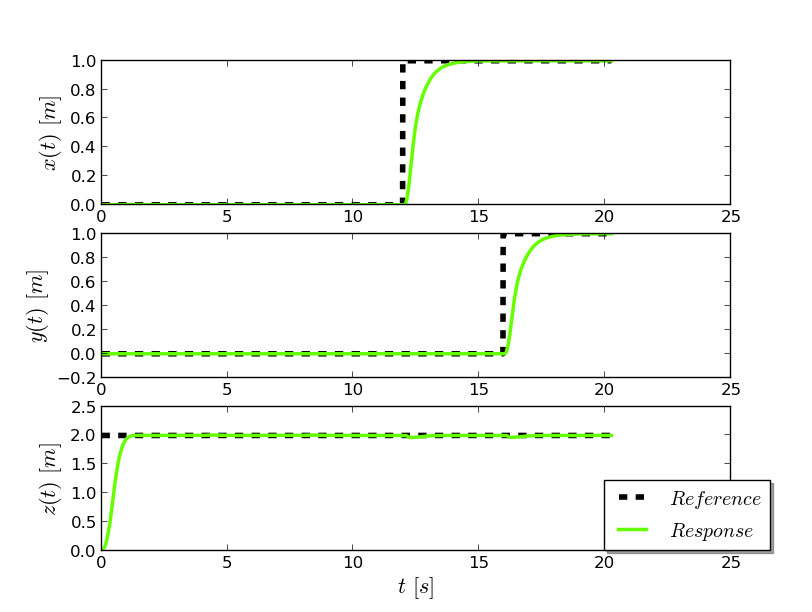
\includegraphics[scale=0.7]{Images/Chapter5/ardrone/position_control.png}
\caption{Trajectory reference and actual trajectory positions of the simulated platform.}
\label{fig:ardrone_pos}
\end{figure}

\begin{figure}[H]
\centering
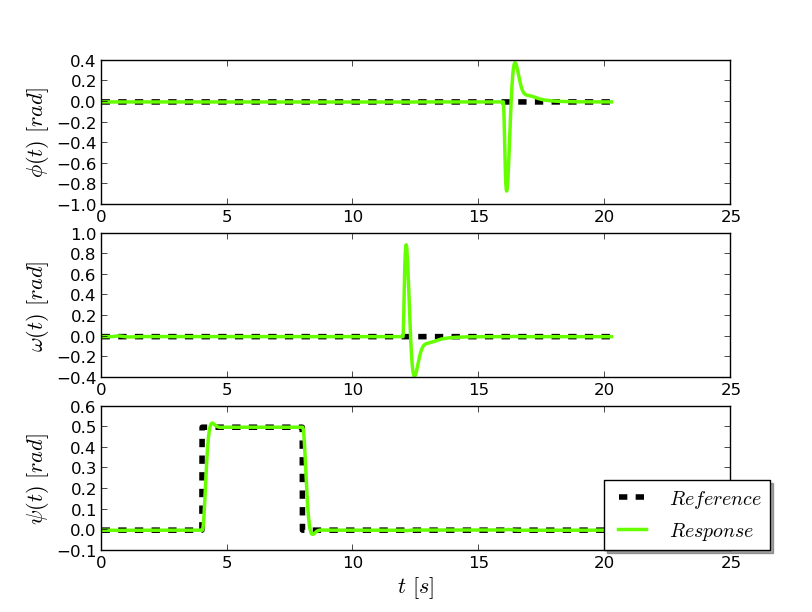
\includegraphics[scale=0.7]{Images/Chapter5/ardrone/euler_angle_control.png}
\caption{Trajectory reference and actual trajectory orientations ($\psi$) of the simulated platform.}
\label{fig:ardrone_ang}
\end{figure}

\begin{figure}[H]
\centering
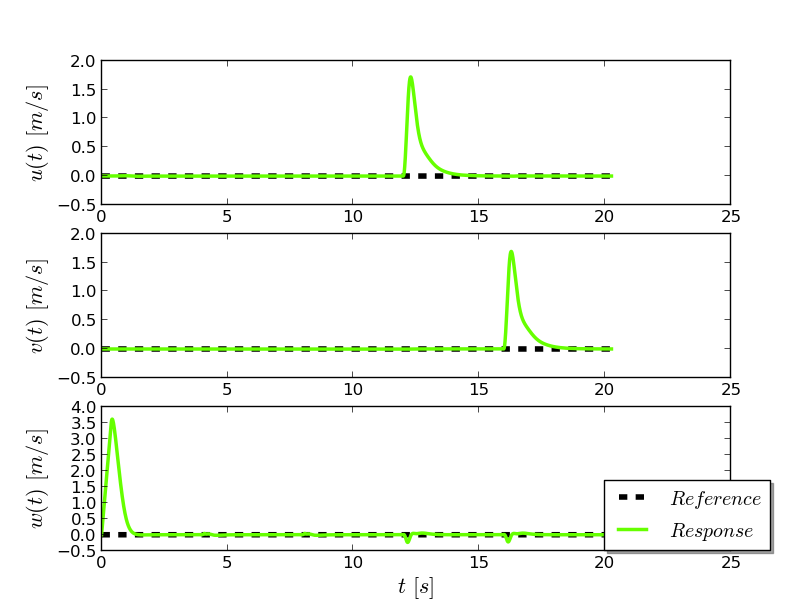
\includegraphics[scale=0.7]{Images/Chapter5/ardrone/lin_velocity_control.png}
\caption{Linear velocities of the simulated platform. }
\label{fig:ardrone_lin_vel}
\end{figure}

\begin{figure}[H]
\centering
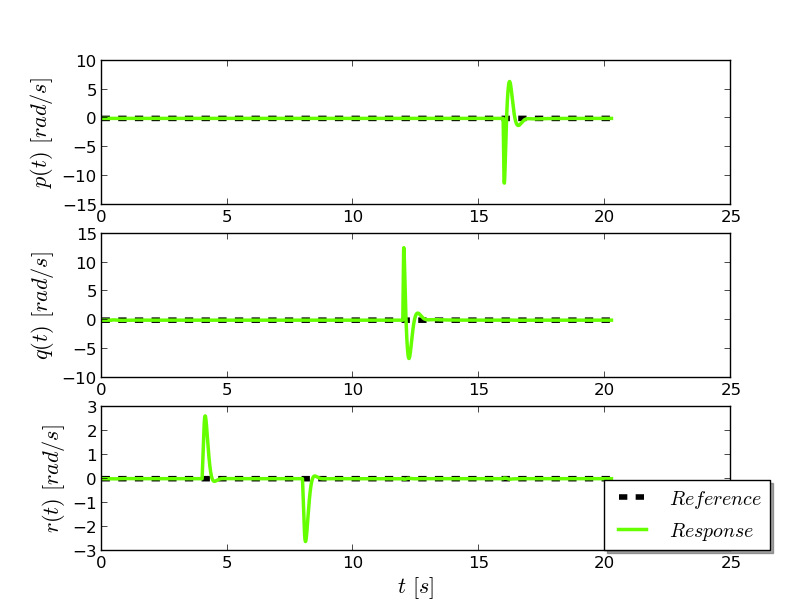
\includegraphics[scale=0.7]{Images/Chapter5/ardrone/ang_velocity_control.png}
\caption{Angular velocities of the simulated platform.}
\label{fig:ardrone_ang_vel}
\end{figure}

\begin{figure}[H]
\centering
\includegraphics[scale=0.7]{Images/Chapter5/ardrone/control_signals_TEST1.png}
\caption{Control signals generated by the MPC strategy.}
\label{fig:ardrone_inputs}
\end{figure}

\subsection{Discussion}

The simulations show the performance of the MPC strategy in the simulated quadrotor. Figures \ref{fig:ardrone_pos} and \ref{fig:ardrone_ang} show the position and orientation  response of the system against step input signals on each controlled variable. The response shown presents a smooth behavior, no overshoot and a small settling time correspondant to a fast system like the quadrotor. The prediction horizon used, $N_p = 30$, has a right balance in speed to allow a fast response without overshoot.\\

The initial set of restrictions considered was bigger than the one used in the simulations shown, since there were restrictions considered on the roll and pitch angles ($\phi$ and $\theta$) taken in order to assure the stability of the quadrotor. Normally, this would be addressed by a hovering PI control loop in the original AR-Drone control architecture. However, the consideration of the constraints on these angles lead to unfeasibility in the quadratic programming problem, so  the correspondant restrictions were relaxed, and eventually dropped. The stability of the platform was addressed by strenghtening the restrictions on the velocities in the $x$ and $y$ axes, since these velocities are dependant on the roll and pitch angles. \\

The actual version of the library does not include functions to cope with unfeasibility. This must be considered in further stages of development in order to provide a better operation under the presence of more constraints. Some suggested strategies to cope with unfeasibility are referred by Camacho and Bordons \cite{CamachoBordons}: an initial strategy consists of dropping the state constraints at the initial portion of the horizon in order to make the problem feasible; another way is to create soft constraints from the hard constraints stated initially, and then adding a term in the cost function to penalize constraint violation \cite{Molero2011}. Feasibility is important to assure closed-loop stability. One could also use the solution of the unconstrained problem  when unfeasibility appears, but this will not guarantee stability. \\

Figure \ref{fig:ardrone_inputs} shows the resultant inputs to the simulator, produced by the optimization solver. As it is shown, the control inputs are only responding to the requirements of the simulation trajectory, hence the regular pattern in the signals. The simulator does not take into account sensor noise or environmental perturbations that can arise such as crossed winds that might require more drastic control inputs to the motors.  \\

To make a verification of the disturbance rejection capabilities of the controller, a test using a disturbance model with a uniform distribution, bounded in a defined range was performed. This disturbance model can not be considered as white gaussian noise that would arise from the sensing instruments, but it works for the aforementioned purpose. In a future work, tests with a disturbance model of the sensor noise and environmental effects on the quadrotor can be performed. These results in a more realistic simulation scenario, would give a better insight of the behavior of the controller in a future implementation on the drone. The bounds of the disturbances were defined to be in the $[0, 0.01]$ range for each state. This affects differently some states, but in general it introduces a slight disturbance without destabilizing the platform. The results of the aforementioned tests are shown below from Figure \ref{fig:ardrone_pos2} to \ref{fig:ardrone_inputs2}.\\

\begin{figure}[H]
\centering
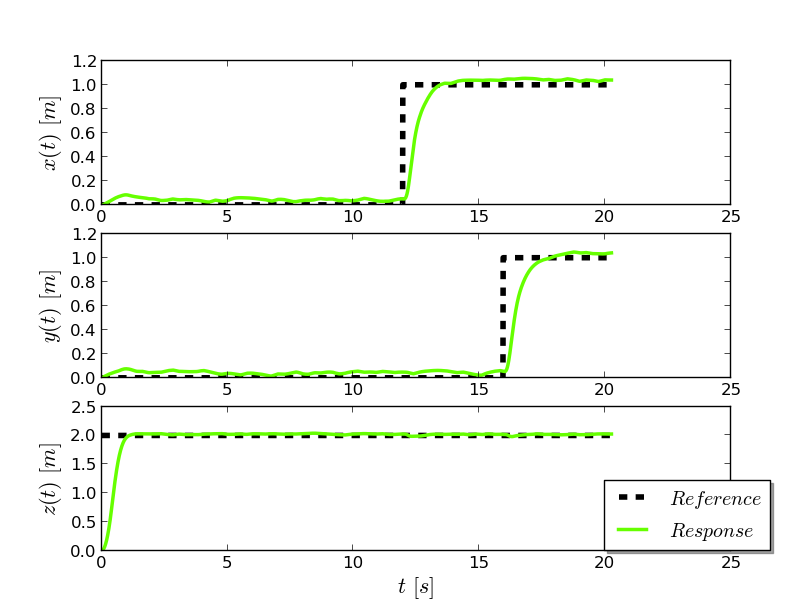
\includegraphics[scale=0.7]{Images/Chapter5/ardrone/T1_noise/position_control.png}
\caption{Trajectory reference and simulated trajectory positions of the platform with the disturbance model.}
\label{fig:ardrone_pos2}
\end{figure}

\begin{figure}[H]
\centering
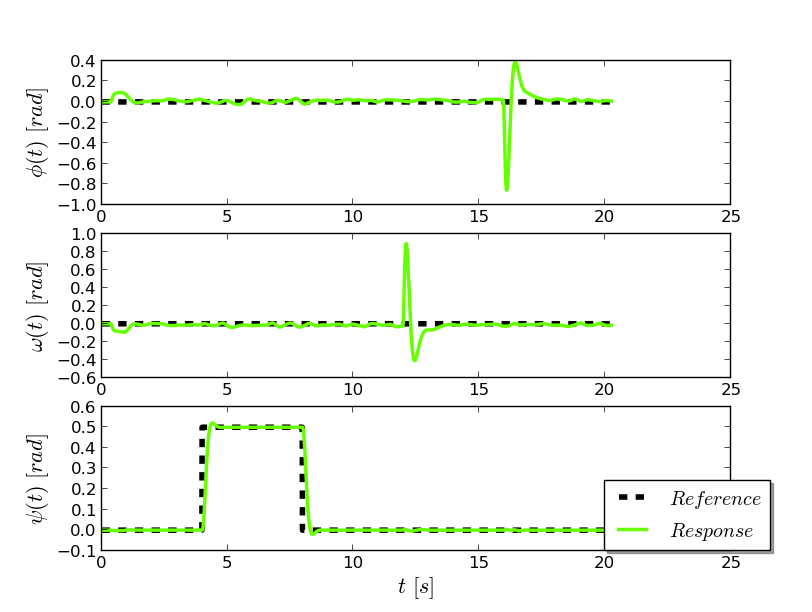
\includegraphics[scale=0.7]{Images/Chapter5/ardrone/T1_noise/euler_angle_control.png}
\caption{Trajectory reference and simulated trajectory orientations ($\psi$) of the platform with the disturbance model.}
\label{fig:ardrone_ang2}
\end{figure}

\begin{figure}[H]    
\centering
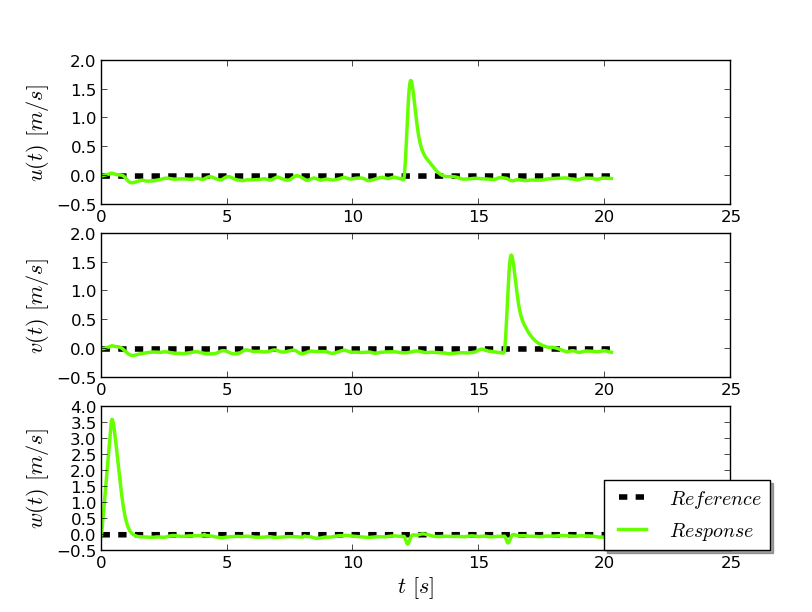
\includegraphics[scale=0.7]{Images/Chapter5/ardrone/T1_noise/lin_velocity_control.png}
\caption{Linear velocities of the simulated platform with the disturbance model. }
\label{fig:ardrone_lin_vel2}
\end{figure}

\begin{figure}[H]
\centering
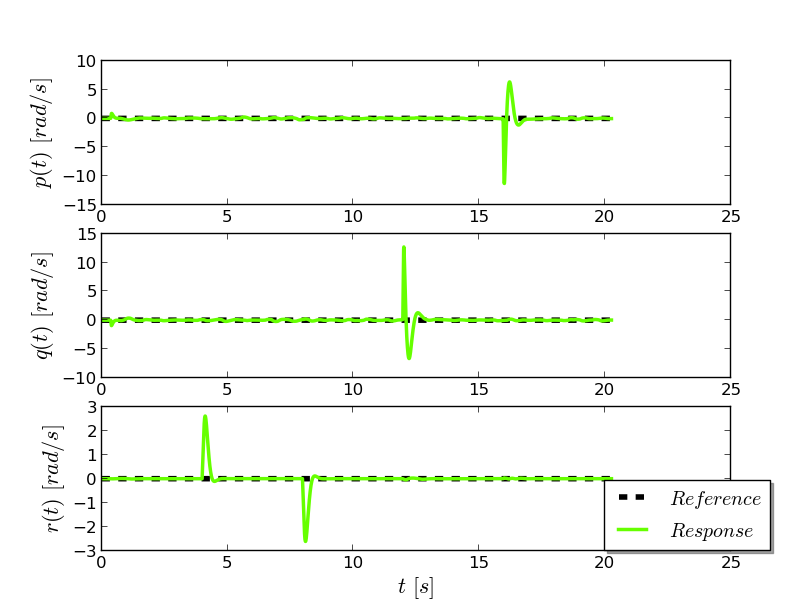
\includegraphics[scale=0.7]{Images/Chapter5/ardrone/T1_noise/ang_velocity_control.png}
\caption{Angular velocities of the simulated platform with the disturbance model.}
\label{fig:ardrone_ang_vel2}
\end{figure}

\begin{figure}[H]
\centering
\includegraphics[scale=0.7]{Images/Chapter5/ardrone/T1_noise/control_signals_TEST2.png}
\caption{Control signals generated by the MPC strategy with the disturbance model.}
\label{fig:ardrone_inputs2}
\end{figure}

The effect of the disturbances is noticeable in Figure \ref{fig:ardrone_inputs2}. With the same disturbance magnitude, there is a slight overshoot in the &X& and &Y& coordinates as Figure \ref{fig:ardrone_pos2} shows, indicating that these are the most sensitive states, since these are critical for the stability of the platform. Despite that, the controller manages to keep the simulated drone stable. This simulation is not performed in real-time, therefore, these results are used to give insight about the proper functionality of the controller instead of the performance. However, the qpOASES solver has a method to limit the computation time of the optimization problem solution to implement it on real-time applications. This allows to obtain suboptimal solutions that can be sufficiently accurate to be implemented in the simulator and also in the real platform. These time cutting methods are not used in this report, but this remains as a topic of interest for an implementation on the quadrotor. In these simulations the computation times for both tests (with and without disturbances) had similar timing, so disturbance rejection seems to not affect this particular topic. The time per iteration in each test is shown below.\\

\begin{center}
    \begin{tabular}{| l | l |}
    \hline
    \textbf{Test} & \textbf{Average Time per MPC iteration} \\ \hline
    Without disturbances & 0.0331 [s]\\ \hline
    With disturbances &  0.0337 [s] \\
    \hline
    \end{tabular}
\end{center}

The simulator was tested in a second trajectory, which is more representative of the kind of motion that the drone would be required to perform in real life applications. It consists in following a square reference of 2 meters of width, one in the horizontal $XY$ plane and one in the vertical &XZ& plane.  The results using this reference are shown below.

\begin{figure}[H]
\centering
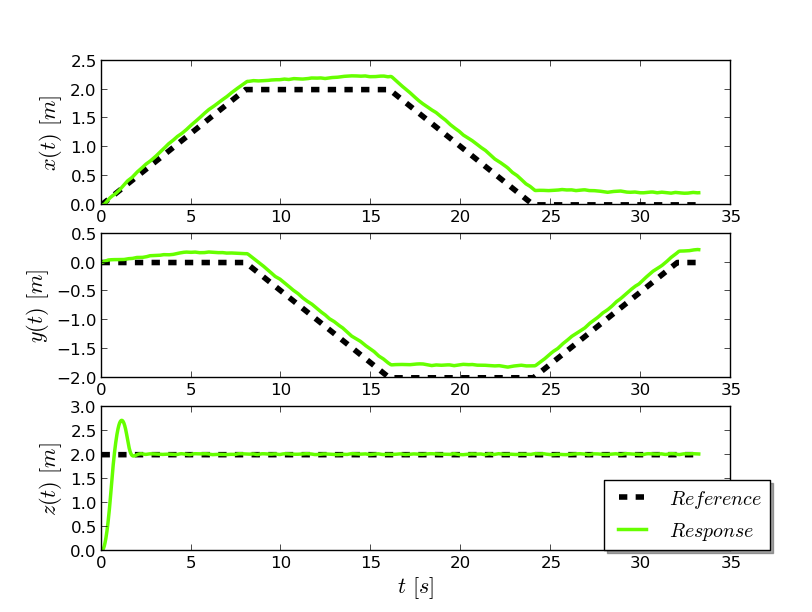
\includegraphics[scale=0.7]{Images/Chapter5/ardrone/T2/position.png}
\caption{Positions of the simulated quadrotor with the square trajectory.}
\label{fig:ardrone_sq_pos}
\end{figure}

\begin{figure}[H]
\centering
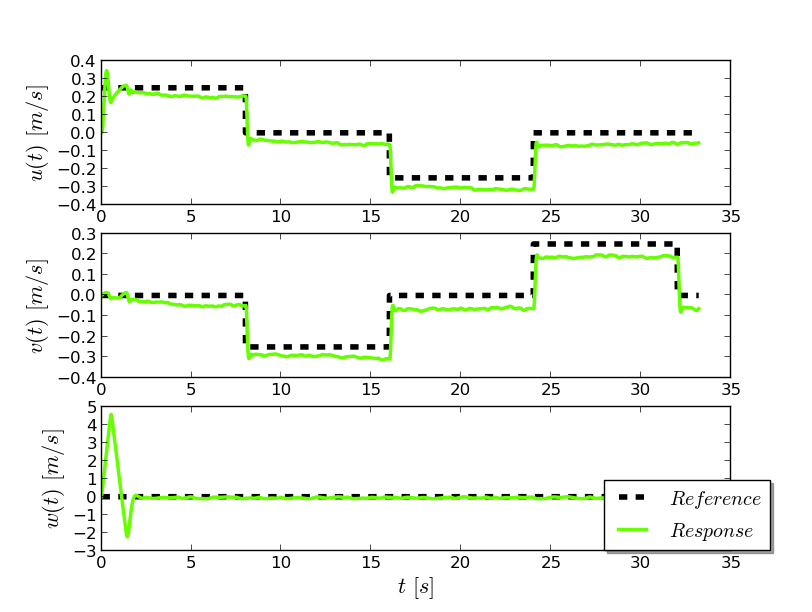
\includegraphics[scale=0.7]{Images/Chapter5/ardrone/T2/velocity.png}
\caption{Linear velocities of the simulated quadrotor with the square trajectory.}
\label{fig:ardrone_sq_vel}
\end{figure}

\begin{figure}[H]    
\centering
\includegraphics[scale=0.7]{Images/Chapter5/ardrone/T2/inputs_TEST3.png}
\caption{Calculated inputs from the MPC to the simulated quadrotor when using the square trajectory. }
\label{fig:ardrone_sq_inp}
\end{figure}

To improve the visualization of these results, the positions are translated into a 2D and 3D space. 

\begin{figure}[H]
        \centering
        \begin{subfigure}[b]{0.5\textwidth}
            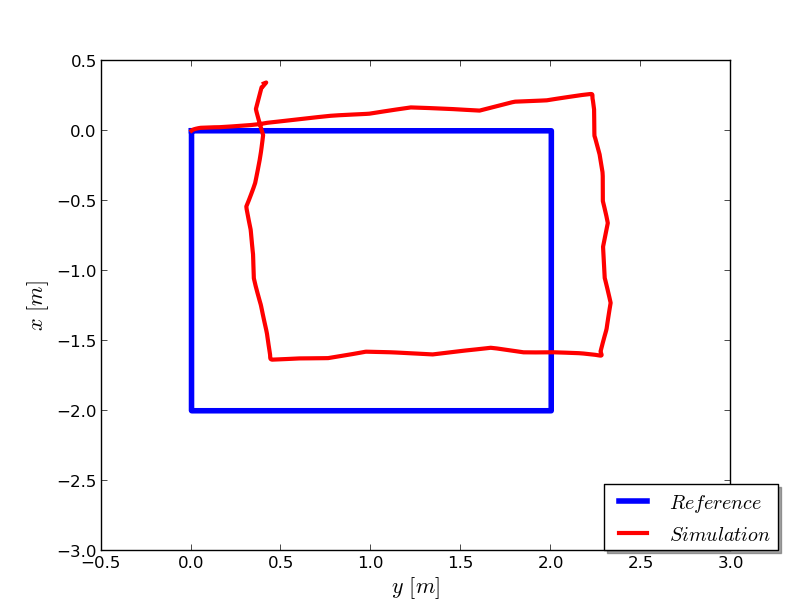
\includegraphics[width=\textwidth]{Images/Chapter5/ardrone/T2/2Dtrajectory.png}   \qquad   
            \caption{Trajectory of the simulated quadrotor in the XY plane.}
            \label{fig:ardrone_sq_2D}  
            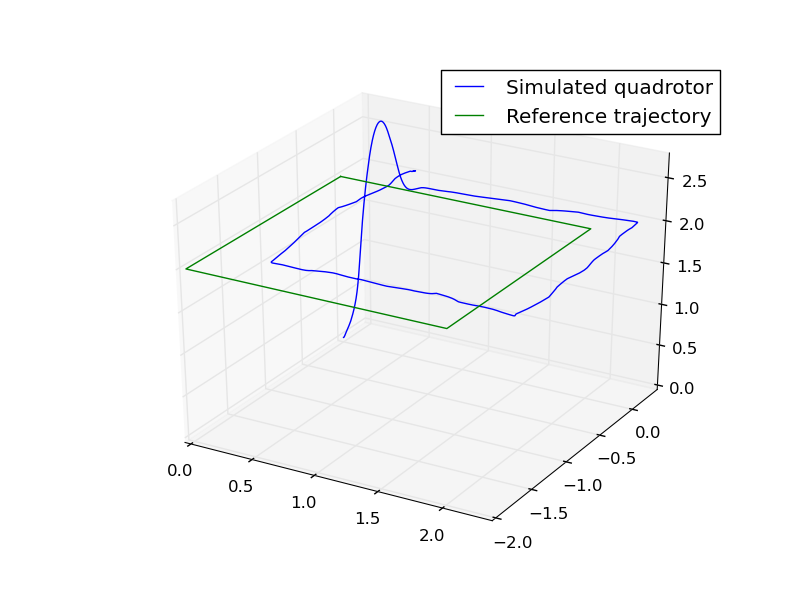
\includegraphics[width=\textwidth]{Images/Chapter5/ardrone/T2/3Dtrajectory.png}
            \caption{Trajectory of the simulated quadrotor in a three dimensional space.}
            \label{fig:ardrone_sq_3D}
        \end{subfigure}
\caption{Visualization of the control trajectories of the simulated platform.}
\label{fig:ardrone_sq_trajectory}
\end{figure}

The previous plots show that the controller performance is not satisfactory. An increasing offset from the desired path appears in the simulation. One reason for this is that the MPC's performance is highly dependant on the accuracy of the model. The model used for this controller is a linear state space representation around the hover point for the quadrotor, which changes immediately after the take off. As the model goes further away from the linearization point, the accuracy of the model decreases respect to the non-linear model, and even more from the real quadrotor. This affects directly the performance of the controller, as the behavior predicted by the model in the MPC drifts away from the simulated behavior of the quadrotor. As model uncertainty increases, it is possible to deal with this situation increasing the restrictions on the system and their correspondent ranges.\\

 However, this approach can easily lead to unfeasibility, as the system becomes overconstrained. In order to improve this, several variants of the MPC algorithm have been studied and implemented to increase its robustness against imperfections in the model and stronger sources of disturbance. Tube MPC \cite{RakovicetAl2010}, is one of these efforts to increase the robustness of the MPC algorithm when uncertainty is present. This variation uses feedback to assure that the states are contained in a tube of possible trajectories. Another fact that must be taken into account to analyze the results, is that the model used in the controller does not count for disturbances. This was not done in this report, but it is of interest to measure the influence of the disturbance model in the development of a model for MPC controllers and their performance. 








  



